\chapter{Extened Gross-Pitaevski equation simulation: GPELAB}
\label{chap:eGPELAB}

In this chapter, we mainly introduce the numerical simulation for quantum droplet. By adding the LHY correction term into the coupled Gross-Pitaevski equation, we can simulate the weak bound droplet with this mean-field 

\section{LHY term of Rb-Na Bose Mixture}
Hamiltonian for BEC with two components is
\begin{equation}
\begin{split}
H_{\text{tot}}=\sum _k \epsilon _{1,k}\hat{a}_{1,k}\dagger\hat{a}_{1,k}+\frac{g_{11}}{2V}\sum _{\left\{k_i\right\}} \hat{a}_{1,k_1}^+\hat{a}_{1,k_2}^+\hat{a}_{1,k_3}\hat{a}_{1,k_4}+\\
\sum_k \epsilon _{2,k}\hat{a}_{2,k}\dagger\hat{a}_{2,k}+\frac{g_{22}}{2V}\sum _{\left\{k_i\right\}} \hat{a}_{2,k_1}^+\hat{a}_{2,k_2}^+\hat{a}_{2,k_3}\hat{a}_{2,k_4}+\frac{g_{12}}{V}\sum
_{\left\{k_i\right\}} \hat{a}_{2,k_1}^+\hat{a}_{1,k_2}^+\hat{a}_{1,k_3}\hat{a}_{2,k_4}
\end{split}
\end{equation}

where \(k_1+k_2=k_3+k_4\), satisfy momentum conservation. \(g_{\text{ii}}\) represent intra-interaction strength, and \(g_{12}\) for inter-interaction.
\(\hat{a}_{i,k}^+\)(\(\hat{a}_{i,k}\)) denote the ladder operator for \(i^{\text{th}}\) component.

\begin{equation}
\begin{split}
\hat{a}_{i,0}=\sqrt{N_i}
\end{split}
\end{equation}

After extended Bogoliubov transformation, we have

\begin{equation}
\begin{split}
H=\frac{g_{11}N_1^2+g_{22}N_2^2+2g_{12}N_1N_2}{2V}+\frac{1}{2}\sum _{k\neq 0} \left(E_++E_--\frac{\hbar ^2k^2}{2m_1}-\frac{\hbar ^2k^2}{2m_2}-\frac{g_{11}N_1+g_{22}N_2}{V}\right)+\\
\sum_{k\neq 0} E_{+,k}\hat{a}_{+,k}\dagger\hat{a}_{+,k}+\sum _{k\neq 0} E_{-,k}\hat{a}_{-,k}\dagger\hat{a}_{-,k}
\end{split}
\end{equation}

where first term gives mean-field ground state energy; second term gives LHY correction; last two terms provide two branches of excitation spectrum.
Details of parameters in above formula are listed here:

\begin{equation}
\begin{split}
E_{\pm }=\sqrt{\frac{\omega _1^2+\omega _2^2}{2}\pm \sqrt{\left(\frac{\omega _1^2-\omega _2^2}{2}\right){}^2+\frac{g_{12}^2N_1N_2}{V^2}\frac{\hbar
^2k^4}{m_1m_2}}}\\
\omega _i=\sqrt{\frac{\hbar ^2k^2}{2m_i}\left(\frac{\hbar ^2k^2}{2m_i}+\frac{2g_{\text{ii}}N_i}{V}\right)}\end{split}
\end{equation}

Ground state energy is
\begin{equation}
\begin{split}
E_{\text{GS}}=\frac{g_{11}N_1^2+g_{22}N_2^2+2g_{12}N_1N_2}{2V}+\\
\frac{1}{2}\sum _{k\neq 0} \left(E_++E_--\frac{\hbar ^2k^2}{2m_1}-\frac{\hbar ^2k^2}{2m_2}-\frac{g_{11}N_1+g_{22}N_2}{V}\right)
\end{split}
\end{equation}

After re-normalization we have the second term, LHY term, which can be rewritten with (4) in

\begin{equation}
\begin{split}
E_{\text{LHY}}&=\frac{1}{2}\sum _{k\neq 0} \left(\sqrt{\frac{\omega _1^2+\omega _2^2}{2}+\sqrt{\left(\frac{\omega _1^2-\omega _2^2}{2}\right){}^2+g_{12}^2n_1n_2\frac{\hbar^4k^4}{m_1m_2}}}+\right.\\
&\left.\sqrt{\frac{\omega _1^2+\omega _2^2}{2}-\sqrt{\left(\frac{\omega _1^2-\omega _2^2}{2}\right){}^2+g_{12}^2n_1n_2\frac{\hbar ^4k^4}{m_1m_2}}}-\frac{\hbar^2k^2}{2m_1}-\frac{\hbar ^2k^2}{2m_2}-g_{11}n_1-g_{22}n_2+\frac{m_1g_{11}^2n_1^2+m_2g_{22}^2n_2^2+4\frac{m_1m_2}{m_1+ m_2}g_{12}^2n_1n_2}{\hbar ^2k^2}\right)
\end{split}
\end{equation}

Replace summation by integral (\(\sum _k \to V\int d\pmb{\overset{\rightharpoonup }{\pmb{k}}}\)), we have

\begin{equation}
\begin{split}
\mathcal{E}_{\text{LHY}}=\frac{E_{\text{LHY}}}{V}=\int _0^{k_c\to  \infty }\frac{k^2}{4\pi ^2}\left(\sqrt{\frac{\omega _1^2+\omega _2^2}{2}+\sqrt{\left(\frac{\omega
_1^2-\omega _2^2}{2}\right){}^2+g_{12}^2n_1n_2\frac{\hbar ^4k^4}{m_1m_2}}}+\right.\\
\left.\sqrt{\frac{\omega _1^2+\omega _2^2}{2}-\sqrt{\left(\frac{\omega _1^2-\omega _2^2}{2}\right){}^2+g_{12}^2n_1n_2\frac{\hbar ^4k^4}{m_1m_2}}}-\frac{\hbar
^2k^2}{2m_1}-\frac{\hbar ^2k^2}{2m_2}-g_{11}n_1-g_{22}n_2+\frac{m_1g_{11}^2n_1^2+m_2g_{22}^2n_2^2+4\frac{m_1m_2}{m_1+ m_2}g_{12}^2n_1n_2}{\hbar ^2k^2}\right)dk
\end{split}
\end{equation}

For simplicity, we reform it into dimensionless form

\begin{equation}
\begin{split}
\mathcal{E}_{\text{LHY}}=C_1\int _0^{k_c}\frac{15}{32}\tilde{k}^2\left(\surd \left(\frac{1}{2}\left( \frac{\tilde{k}^2}{2}\left(\frac{\tilde{k}^2}{2}+2\right)+\frac{1}{\gamma
^2}\frac{\tilde{k}^2}{2}\left(\frac{\tilde{k}^2}{2}+2y \gamma \right)\right)+\sqrt{\left(\frac{1}{2}\left( \frac{\tilde{k}^2}{2}\left(\frac{\tilde{k}^2}{2}+2\right)-\frac{1}{\gamma
^2}\frac{\tilde{k}^2}{2}\left(\frac{\tilde{k}^2}{2}+2y \gamma \right)\right)\right)^2+\frac{x y}{\gamma }\tilde{k}^4}\right)+\right.\\
\left.\surd \left(\frac{1}{2}\left( \frac{\tilde{k}^2}{2}\left(\frac{\tilde{k}^2}{2}+2\right)+\frac{1}{\gamma ^2}\frac{\tilde{k}^2}{2}\left(\frac{\tilde{k}^2}{2}+2y
\gamma \right)\right)-\sqrt{\left(\frac{1}{2}\left( \frac{\tilde{k}^2}{2}\left(\frac{\tilde{k}^2}{2}+2\right)-\frac{1}{\gamma ^2}\frac{\tilde{k}^2}{2}\left(\frac{\tilde{k}^2}{2}+2y
\gamma \right)\right)\right)^2+\frac{x y}{\gamma }\tilde{k}^4}\right)-\frac{\tilde{k}^2}{2}\left(1+\frac{1}{\gamma }\right)-1-y+\frac{1+\gamma  y^2+\frac{4x
y \gamma }{1+\gamma }}{\tilde{k}^2}\right)d\tilde{k}
\end{split}
\end{equation}

where

\begin{equation}
\begin{split}
C_1=\frac{8}{15\pi ^2}g_{11}n_1\left(\frac{\sqrt{m_1g_{11}n_1}}{\hbar }\right){}^3, \gamma =\frac{m_2}{m_1}, x=\frac{g_{12}^2}{g_{11}g_{22}}, y=\frac{g_{22}n_2}{g_{11}n_1},
\tilde{k}=\frac{\hbar  k}{\sqrt{m_1g_{11}n_1}}
\end{split}
\end{equation}

using \(f\left(\frac{m_2}{m_1},\frac{g_{12}^2}{g_{11}g_{22}},\frac{g_{22}n_2}{g_{11}n_1}\right)\) replacing the tedious integral, we have

\begin{equation}
\begin{split}
\mathcal{E}_{\text{LHY}}=\frac{8}{15\pi ^2}\frac{m_1^{3/2}\left(g_{11}n_1\right){}^{5/2}}{\hbar ^3}f(\gamma ,x,y)
\end{split}
\end{equation}

\section{Calculation(\textit{ calculated by MMA, not full spectrum})}

In this section, we will calculate \(f(\gamma ,x,y)\) numerically for our Rb-Na Bose mixture system

First we do this integration and check its convergence. We plot \(f(\gamma ,x,y)\) with increasing upper bound of integration \(k_C\) to test its
convergence.

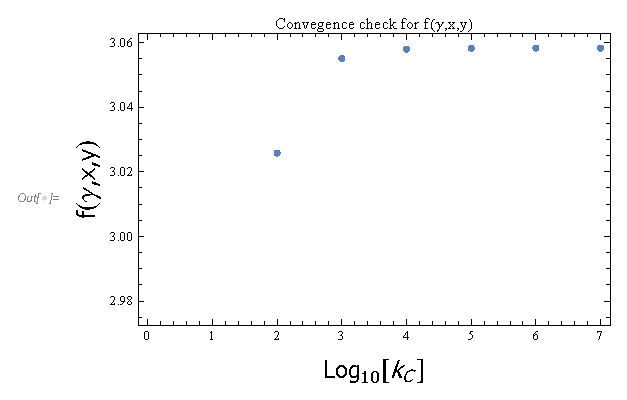
\includegraphics{Note_GPELAB_Droplet_gr1.eps}

We can say that integration up to order of 6 has converged. 
Then, we calculate \(f(\gamma ,x,y)\) with different \(x\), i.e. with different B-field Compared with Minardi{'}s approximation \cite{Minardi2019}, they propose a analytical approximation which will be more convenient for deriving GPE with LHY correction. Here is the formula:
\begin{equation}
\begin{split}
f(z,u=1,x)\simeq \left(1+z^{3/5}x\right)^{5/2}
\end{split}
\end{equation}
where
\begin{equation}
\begin{split}
z=m_2/m_1, x=\frac{g_{22}n_2}{g_{11}n_1},u=\frac{g_{12}^2}{g_{11}g_{22}}
\end{split}
\end{equation}

Here, \(u\) is set to be 1.
Now, we compare the numerical solution with the Minardi{'}s approximation.
Plot of List of f($\gamma $,x,y) for numerical one and Minardi{'}s approximation.

ADD FORMULAS

So, we can see that, there are mainly several percentage error by using this formula. And the maximum error is about 15$\%$. So, keep this error in mind about the LHY energy.

\section{Derivation of GPE and extendedGPE from mean-field energy}

First, we assume the many-body wave function is a product state

\begin{equation}
\begin{split}
\Psi \left(\overset{\rightharpoonup }{r}_1,\overset{\rightharpoonup }{r}_2,\ldots  ,\overset{\rightharpoonup }{r}_N\right)=\sum _{i=1}^N \psi \left(\overset{\rightharpoonup
}{r}_i\right)
\end{split}
\end{equation}

Then, we have

\begin{equation}
\begin{split}
E\left(\psi ,\psi ^*\right)=N\int dr^3\left(\frac{\hbar ^2}{2m}\left| \nabla \psi (r)\right| ^2+V(r)\left| \psi (r)\right| ^2+\frac{1}{2}N g\left|
\psi (r)\right| ^4\right)
\end{split}
\end{equation}

define the Variation

\begin{equation}
\begin{split}
X\left(\psi ,\psi ^*\right)=E\left(\psi ,\psi ^*\right)-\mu  N\int dr^3\left| \psi (r)\right| ^2
\end{split}
\end{equation}

take the variation of \(X\left(\psi ,\psi ^*\right)\), we have

\begin{equation}
\begin{split}
\delta  X\left(\psi ,\psi ^*\right)=N\int dr^3\left(\frac{\hbar ^2}{2m}\left(\nabla \psi ^*(r)\nabla \delta \psi (r)+\nabla \psi (r)\nabla \delta
\psi ^*(r)\right)+(V(r)-\mu )\left(\psi ^*(r)\delta  \psi (r)+\psi (r)\delta  \psi ^*(r) \right)+N g\left(\psi ^2(r)\delta  \psi ^*(r)+\psi ^*^2(r)\delta
 \psi (r)\right)\right)\\
=N\int dr^3\left(\frac{\hbar ^2}{2m}\left(\nabla \psi (r)\nabla \delta \psi ^*(r)\right)+(V(r)-\mu )\left(\psi (r)\delta  \psi ^*(r) \right)+N g\left(\psi
^2(r)\psi ^*(r)\delta  \psi ^*(r)\right)\right)+c.c.
\end{split}
\end{equation}

for the first part, by using integrating by part method:

\begin{equation}
\begin{split}
\int dr^3\left(\nabla \psi (r)\nabla \delta \psi ^*(r)\right)=\delta \psi ^*(r)\nabla \psi (r)|_0^{\infty }-\int dr^3\left(\nabla ^2\psi (r)\delta
\psi ^*(r)\right)=\int dr^3\left(-\nabla ^2\psi (r)\right)\delta \psi ^*(r)
\end{split}
\end{equation}

Them, take the variance to be zero, we have GPE

\begin{equation}
\begin{split}
-\frac{\hbar ^2}{2m}\left(\nabla ^2\psi (r)\right)+(V(r)-\mu )\psi (r)+N g\left(\psi ^2(r)\psi ^*(r)\right)=0\\
-\frac{\hbar ^2}{2m}\left(\nabla ^2\psi ^*(r)\right)+(V(r)-\mu )\psi ^*(r)+N g\left(\psi ^*^2(r)\psi (r)\right)=0
\end{split}
\end{equation}

First, we assume the many-body wave function is a product state

\begin{equation}
\begin{split}
\Psi \left(\overset{\rightharpoonup }{r}_1,\overset{\rightharpoonup }{r}_2,\ldots  ,\overset{\rightharpoonup }{r}_N\right)=\sum _{i=1}^N \psi \left(\overset{\rightharpoonup
}{r}_i\right)
\end{split}
\end{equation}

Then, we have

\begin{equation}
\begin{split}
E\left(\psi ,\psi ^*\right)=N\int dr^3\left(\frac{\hbar ^2}{2m}\left(\nabla \psi ^*(r)\nabla \psi (r)\right)+V(r)\left(\psi ^*(r)\psi (r)\right)+\frac{1}{2}N
g\left(\psi ^*(r)\psi (r)\right)^2+C \left(\psi ^*(r)\psi (r)\right)^{5/2}\right)
\end{split}
\end{equation}

define the Variation

\begin{equation}
\begin{split}
X\left(\psi ,\psi ^*\right)=E\left(\psi ,\psi ^*\right)-\mu  N\int dr^3\left(\psi ^*(r)\psi (r)\right)
\end{split}
\end{equation}

take the variation of \(X\left(\psi ,\psi ^*\right)\), we have

\begin{equation}
\begin{split}
\delta  X\left(\psi ,\psi ^*\right)=N\int dr^3\left(\frac{\hbar ^2}{2m}\left(\nabla ^2\psi (r)\delta \psi ^*(r)\right)+(V(r)-\mu )\left(\psi (r)\delta
\psi ^*(r) \right)+N g\left(\psi ^2(r)\psi ^*(r)\delta \psi ^*(r)\right)+\frac{5C}{2}(\psi (r))^{5/2}\left(\psi ^*(r)\right)^{3/2}\delta \psi ^*(r)\right)+c.c.
\end{split}
\end{equation}

where C is constants which already expressed the Last Part.
thus, we have eGPE

\begin{equation}
\begin{split}
-\frac{\hbar ^2}{2m}\left(\nabla ^2\psi (r)\right)+(V(r)-\mu )\psi (r)+N g\left(\psi ^*(r)\psi (r)\right)\psi (r)+\frac{5C}{2}\left(\psi (r)\psi
^*(r)\right)^{3/2}\psi (r)=0\\
-\frac{\hbar ^2}{2m}\left(\nabla ^2\psi ^*(r)\right)+(V(r)-\mu )\psi ^*(r)+N g\left(\psi ^*^2(r)\psi (r)\right)+\frac{5C}{2}\left(\psi ^*(r)\right)^{5/2}(\psi
(r))^{3/2}=0
\end{split}
\end{equation}

First, we assume the many-body wave function is a product state

\begin{equation}
\begin{split}
\Psi \left(\overset{\rightharpoonup }{r}_1,\overset{\rightharpoonup }{r}_2,\ldots  ,\overset{\rightharpoonup }{r}_N\right)=\sum _{i=1}^N \psi _1\left(\overset{\rightharpoonup
}{r}_i\right)\sum _{i=1}^N \psi _2\left(\overset{\rightharpoonup }{r}_i\right)
\end{split}
\end{equation}

Then, we have

\begin{equation}
\begin{split}
E\left(\psi _1,\psi _1{}^*,\psi _2,\psi _2{}^*\right)=\int dr^3\left(
\begin{array}{cc}
 \psi _1^* & \psi _2^* \\
\end{array}
\right).\left(
\begin{array}{cc}
 \mathcal{H}_{11} & \mathcal{H}_{12} \\
 \mathcal{H}_{21} & \mathcal{H}_{22} \\
\end{array}
\right).\left(
\begin{array}{c}
 \psi _1 \\
 \psi _2 \\
\end{array}
\right)+E_{\text{LHY}}
\end{split}
\end{equation}

where \(\mathcal{H}_{ij}\) represent the Hamiltonian density of fields

\begin{equation}
\begin{split}
\mathcal{H}_{11}=N_1\left(\frac{\hbar ^2}{2m_1}(\nabla )^2+V_1(r)+\frac{1}{2}N_1g_{11}\left(\psi _1{}^*(r)\psi _1(r)\right)\right)\\
\mathcal{H}_{22}=N_2\left(\frac{\hbar ^2}{2m_2}(\nabla )^2+V_2(r)+\frac{1}{2}N_2g_{22}\left(\psi _2{}^*(r)\psi _2(r)\right){}^2\right)\\
\mathcal{H}_{12}=\mathcal{H}_{21}^{\dagger }=N_1N_2g_{12}\left(\psi _1{}^*(r)\psi _1(r)\right)\left(\psi _2{}^*(r)\psi _2(r)\right)
\end{split}
\end{equation}

and LHY term has been expressed in the last part.
define the Variation

\begin{equation}
\begin{split}
X\left(\psi ,\psi ^*\right)=E\left(\psi ,\psi ^*\right)-\mu _1 N_1\int dr^3\left(\psi _1{}^*(r)\psi _1(r)\right)-\mu _2 N_2\int dr^3\left(\psi
_2{}^*(r)\psi _2(r)\right)
\end{split}
\end{equation}

Finally, we have eGPE for 

\begin{equation}
\begin{split}
i \hbar \frac{\partial \psi _1}{\partial t}=\left(-\frac{\hbar ^2\nabla ^2}{2m_1}+V_1+g_{11}n_1+g_{12}n_2+\frac{\delta  \mathcal{E}_{\text{LHY}}}{\delta
 n_1}\right)\psi _1\\
i \hbar \frac{\partial \psi _2}{\partial t}=\left(-\frac{\hbar ^2\nabla ^2}{2m_2}+V_2+g_{22}n_2+g_{12}n_1+\frac{\delta  \mathcal{E}_{\text{LHY}}}{\delta
 n_2}\right)\psi _2
\end{split}
\end{equation}

\section{eGPE for GPELAB with Minardi approximation}

\begin{equation}
\begin{split}
i \hbar \frac{\partial \psi _1}{\partial t}=\left(-\frac{\hbar ^2\nabla ^2}{2m_1}+V_1+g_{11}n_1+g_{12}n_2+\frac{\delta  \mathcal{E}_{\text{LHY}}}{\delta
 n_1}\right)\psi _1\\
i \hbar \frac{\partial \psi _2}{\partial t}=\left(-\frac{\hbar ^2\nabla ^2}{2m_2}+V_2+g_{22}n_2+g_{12}n_1+\frac{\delta  \mathcal{E}_{\text{LHY}}}{\delta
 n_2}\right)\psi _2
\end{split}
\end{equation}

where
\(n_i=N_i\psi _i^*\psi _i=N_i|\psi _i|^2\)
and 

\begin{equation}
\begin{split}
\frac{\delta  \mathcal{E}_{\text{LHY}}}{\delta  n_1}=\frac{8}{15\pi ^2}\frac{m_1^{3/2}\left(g_{11}\right){}^{5/2}n_1^{1/2}}{\hbar ^3}\left(\frac{5}{2}n_1f(\gamma
,x,y)-\frac{g_{22}n_2}{g_{11}}\frac{\partial f(\gamma ,x,y)}{\partial y}\right)
\end{split}
\end{equation}

\begin{equation}
\begin{split}
\frac{\delta  \mathcal{E}_{\text{LHY}}}{\delta  n_2}=\frac{8}{15\pi ^2}\frac{m_1^{3/2}\left(g_{11}\right){}^{3/2}g_{22}n_1^{3/2}}{\hbar ^3}\frac{\partial
f(\gamma ,x,y)}{\partial y}
\end{split}
\end{equation}

if we using the approximation formula, we have

\begin{equation}
\begin{split}
\mathcal{E}_{\text{LHY}}=\frac{8}{15\pi ^2}\frac{m_1^{3/2}\left(g_{11}n_1\right){}^{5/2}}{\hbar ^3}\left(1+\gamma ^{3/5}y\right)^{5/2}
\end{split}
\end{equation}

Then, 

\begin{equation}
\begin{split}
\frac{\delta  \mathcal{E}_{\text{LHY}}}{\delta  n_1}=\frac{8}{15\pi ^2}\frac{m_1^{3/2}\left(g_{11}\right){}^{5/2}n_1^{1/2}}{\hbar ^3}\left(\frac{5}{2}n_1\left(1+\gamma
^{3/5}y\right){}^{5/2}-\frac{5}{2}\frac{g_{22}n_2}{g_{11}}\left(1+\gamma ^{3/5}y\right)^{3/2}\gamma ^{3/5}\right)\\
=\frac{4}{3\pi ^2}\frac{m_1^{3/2}\left(g_{11}\right){}^{5/2}n_1^{3/2}}{\hbar ^3}\left(1+\gamma ^{3/5}y\right)^{3/2}
\end{split}
\end{equation}

\begin{equation}
\begin{split}
\frac{\delta  \mathcal{E}_{\text{LHY}}}{\delta  n_2}=\frac{8}{15\pi ^2}\frac{m_1^{3/2}\left(g_{11}\right){}^{3/2}g_{22}n_1^{3/2}}{\hbar ^3}\frac{5}{2}\left(1+\gamma
^{3/5}y\right)^{3/2}\gamma ^{3/5}\\
=\frac{4}{3\pi ^2}\frac{\gamma ^{3/5}m_1^{3/2}\left(g_{11}\right){}^{3/2}g_{22}n_1^{3/2}}{\hbar ^3}\left(1+\gamma ^{3/5}y\right)^{3/2}
\end{split}
\end{equation}

Finally, we have extended GPE as

\begin{equation}
\begin{split}
i \hbar \frac{\partial \psi _1}{\partial t}=\left(-\frac{\hbar ^2\nabla ^2}{2m_1}+V_1+g_{11}n_1+g_{12}n_2+\frac{4}{3\pi ^2}\frac{g_{11}m_1^{3/5}}{\hbar
^3}\left(g_{11}n_1m_1^{3/5}+g_{22}n_2m_2^{3/5}\right){}^{3/2}\right)\psi _1\\
i \hbar \frac{\partial \psi _2}{\partial t}=\left(-\frac{\hbar ^2\nabla ^2}{2m_2}+V_2+g_{22}n_2+g_{12}n_1+\frac{4}{3\pi ^2}\frac{g_{22}m_2^{3/5}}{\hbar
^3}\left(g_{11}n_1m_1^{3/5}+g_{22}n_2m_2^{3/5}\right){}^{3/2}\right)\psi _2
\end{split}
\end{equation}

Now, we need do DimensionReduction, 

\begin{equation}
\begin{split}
i \frac{\partial \Psi _1}{\partial T}=\left(-\frac{m\pmb{\nabla }^2}{2m_1}+\frac{V_1}{\hbar  \omega }+4\pi  \frac{m}{m_1}\frac{ N_1a_{11}}{a}\Psi
_1^*\Psi _1+2\pi \frac{ m }{m_{12}}\frac{N_2a_{12}}{a}\Psi _2^*\Psi _2+\frac{128\pi ^{1/2} }{3} \frac{a_{11}}{a}\left(\frac{m}{m_1}\right){}^{2/5}\left(
\frac{N_1a_{11}}{a}\left(\frac{m}{m_1}\right){}^{2/5}\Psi _1^*\Psi _1+ \frac{N_2a_{22}}{a}\left(\frac{m}{m_2}\right){}^{2/5}\Psi _2^*\Psi _2\right){}^{3/2}\right)\Psi
_1\\
i \frac{\partial \Psi _2}{\partial T}=\left(-\frac{m\pmb{\nabla }^2}{2m_2}+\frac{V_2}{\hbar  \omega }+4\pi  \frac{m}{m_2}\frac{\text{  }N_2a_{22}}{a}\Psi
_2^*\Psi _2+2\pi \frac{ m }{m_{12}}\frac{N_1a_{12}}{a}\Psi _1^*\Psi _1+\frac{128\pi ^{1/2} }{3}\frac{a_{22}}{a}\left(\frac{m}{m_2}\right){}^{2/5}\left(
\frac{N_1a_{11}}{a}\left(\frac{m}{m_1}\right){}^{2/5}\Psi _1^*\Psi _1+ \frac{N_2a_{22}}{a}\left(\frac{m}{m_2}\right){}^{2/5}\Psi _2^*\Psi _2\right){}^{3/2}\right)\Psi
_2
\end{split}
\end{equation}

where we set \(V_1\) and \(V_2\) as harmonic trap, and it gives the characteristic length and time. Actually, this characteristic length and time
can be arbitrary.

\begin{equation}
\begin{split}
g_{11}=\frac{4\pi  \hbar ^2a_{11}}{m_1}, g_{22}=\frac{4\pi  \hbar ^2a_{22}}{m_2}, g_{12}=\frac{2\pi  \hbar ^2a_{12}}{m_{12}}, m_{12}=\frac{m_1m_2}{m_1+m_2}\\
T=\omega  t, \overset{\rightharpoonup }{R}=\left.\overset{\rightharpoonup }{r}\right/a, \Psi =\psi  a^{3/2}, a=\sqrt{\frac{\hbar }{m \omega }}
\end{split}
\end{equation}

By the way, we can calculate the Nonlinear-Energy function. (Just for fun, not for GPELAB)

Recall LHY energy term

\begin{equation}
\begin{split}
\mathcal{E}_{\text{LHY}}=\frac{8}{15\pi ^2}\frac{m_1^{3/2}\left(g_{11}n_1\right){}^{5/2}}{\hbar ^3}\left(1+\left(\frac{m_2}{m_1}\right){}^{3/5}\frac{g_{22}n_2}{g_{11}n_1}\right){}^{5/2}\\
=\frac{256\sqrt{\pi }\hbar ^2}{15}\left(m_1^{-2/5}a_{11}n_1+m_2^{-2/5}a_{22}n_2\right){}^{5/2}
\end{split}
\end{equation}

Do DimensionReduction, we have

\begin{equation}
\begin{split}
\frac{\mathcal{E}_{\text{LHY}}}{\hbar  \omega \left/a^3\right.}=\frac{256\pi ^{1/2}}{15}\left(\frac{N_1a_{11}}{a}\left(\frac{m}{m_1}\right){}^{2/5}\Psi
_1^*\Psi _1+ \frac{N_2a_{22}}{a}\left(\frac{m}{m_2}\right){}^{2/5}\Psi _2^*\Psi _2\right){}^{5/2}
\end{split}
\end{equation}
